\section{Model Learning \& Optimization}

\begin{frame}
\frametitle{Mobile Robot Navigation}
\textcolor{tudblue}{\textbf{Goal:}} Move robot to area while minimizing traveled distance
\vfill

\begin{columns}[T]
\begin{column}{0.5\textwidth}
MDP Model $\mathcal{M}$ should define:
\begin{itemize}
	\item States \hspace{12.75pt}$\mapsto$ locations
	\item Actions \hspace{7.5pt}$\mapsto$ robot translations
	\item Rewards $\mapsto$ goal areas
	\item Transition-function
\end{itemize}

\end{column}

\begin{column}{0.425\textwidth}
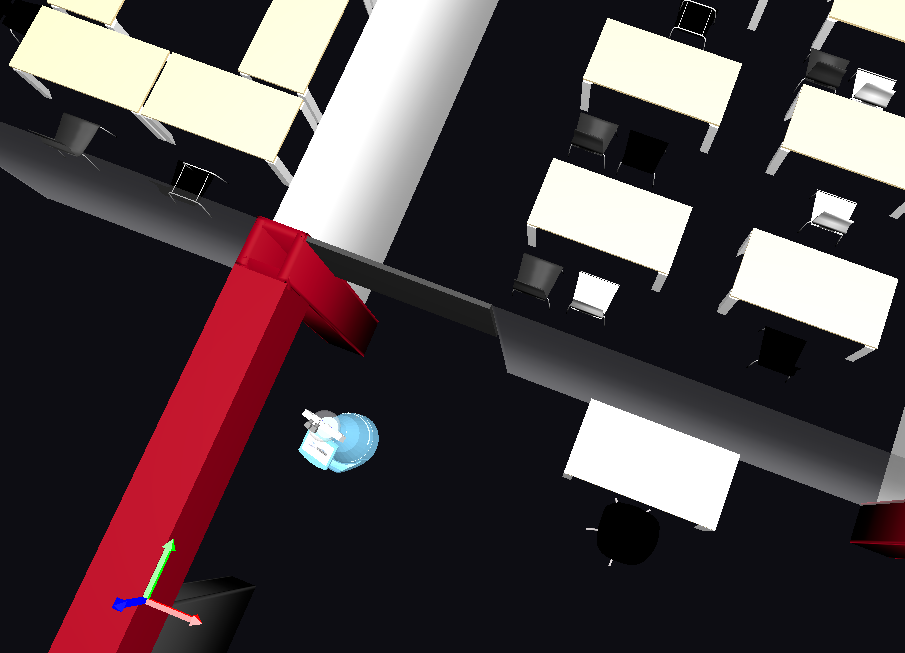
\includegraphics[width=\textwidth]{figures/simulator_6_crop}
\end{column}

\end{columns}

\end{frame}

\begin{frame}
\frametitle{Model-Learning for Mobile Robot Navigation}

\begin{columns}[T]
\begin{column}{0.6\textwidth}
\begin{itemize}
	\item Existing approaches for state-space acquisition:
	\begin{itemize}
		\item Grid Discretization
		\item Best-First Model Merging % TODO Add cite
		\item State-Merging by Trajectory Clustering % TODO Add cite
	\end{itemize}
	\item \textbf{TODO}
	\item Simulation in Morse with a Scitos A5 robot
\end{itemize}
\end{column}
\begin{column}{0.5\textwidth}
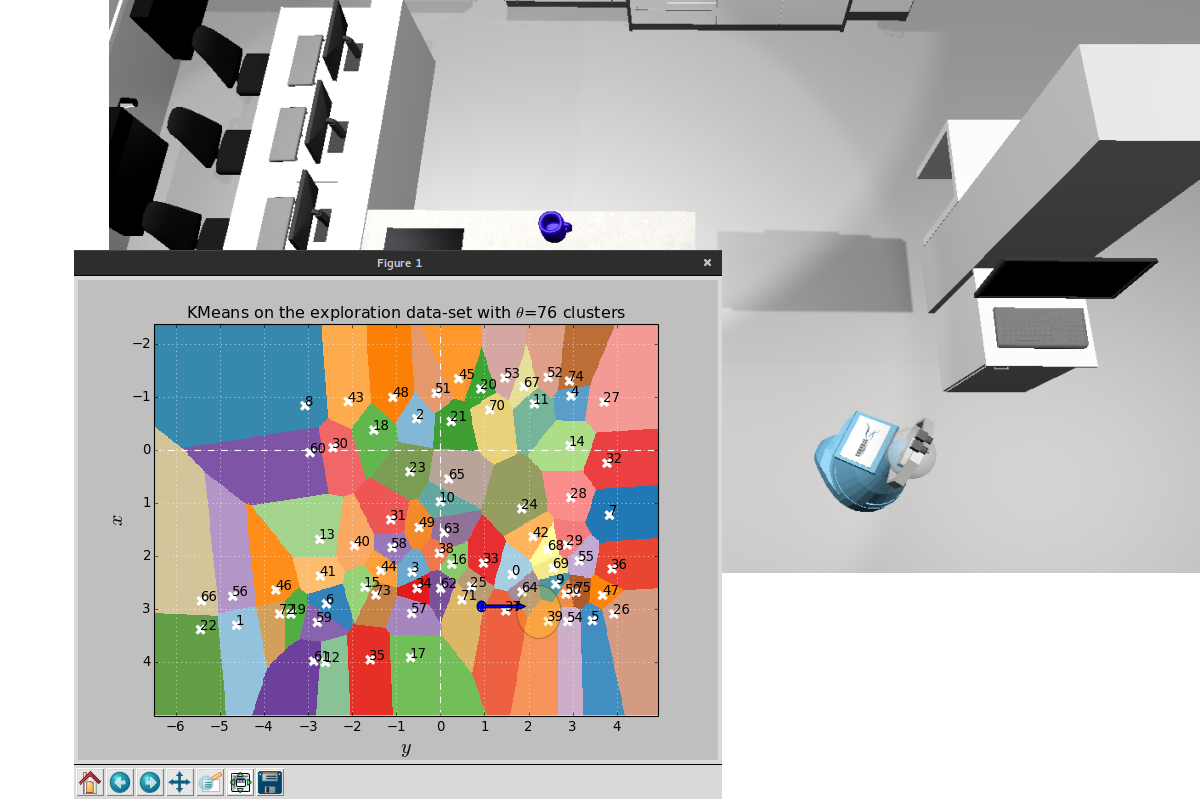
\includegraphics[width=\textwidth, left]{figures/simulation_learn_2}
\end{column}
\end{columns}	
	
\end{frame}

\begin{frame}
\frametitle{Model-Optimization Routine}
\begin{center}
\includegraphics<1| handout:0>[width=1\textwidth]{figures/optimization-routine/learning-cycle-1.pdf}
\includegraphics<2| handout:0>[width=1\textwidth]{figures/optimization-routine/learning-cycle-2.pdf}
\includegraphics<3| handout:0>[width=1\textwidth]{figures/optimization-routine/learning-cycle-3.pdf}
\includegraphics<4| handout:0>[width=1\textwidth]{figures/optimization-routine/learning-cycle-4.pdf}
\includegraphics<5>[width=1\textwidth]{figures/optimization-routine/learning-cycle-5.pdf}
\end{center}
\end{frame}

\begin{frame}
\frametitle{Model-Optimization Routine}
\begin{center}
	\includegraphics<1| handout:0>[width=1\textwidth]{figures/optimization-routine/learning-cycle-simplified-1.pdf}
	\includegraphics<2| handout:0>[width=1\textwidth]{figures/optimization-routine/learning-cycle-simplified-2.pdf}
	\includegraphics<3>[width=1\textwidth]{figures/optimization-routine/learning-cycle-simplified-3.pdf}
\end{center}
\end{frame}